\documentclass[../notes.tex]{subfiles}

\pagestyle{main}
\renewcommand{\chaptermark}[1]{\markboth{\chaptername\ \thechapter\ (#1)}{}}

\begin{document}




\chapter{Classifying Complex Functions}
\section{Holomorphic Functions}
\begin{itemize}
    \item \marginnote{3/19:}We begin by reviewing some properties of the \textbf{complex numbers}.
    \item \textbf{Complex numbers}: The field of elements $z=x+iy$ where $x,y\in\R$ and $i^2=-1$. \emph{Denoted by} $\pmb{\C}$.
    \begin{figure}[h!]
        \centering
        \begin{tikzpicture}[
            every node/.style=black
        ]
            \small
            \draw [-stealth] (-1.5,0) -- (1.5,0) node[right]{$\R$};
            \draw [-stealth] (0,-1.5) -- (0,1.5) node[above]{$i\R$};

            \footnotesize
            \draw (1,0.1)    -- ++(0,-0.2) node[below]{$x$};
            \draw (0.1,0.8)  -- ++(-0.2,0) node[left] {$y$};
            \draw (0.1,-0.8) -- ++(-0.2,0) node[left] {$-y$};

            \fill [rex] (1,0.8)  coordinate (z)    circle (1.5pt) node[above right]{$z$};
            \fill [rex] (1,-0.8) coordinate (zbar) circle (1.5pt) node[below right]{$\bar{z}$};
            \draw [rex,semithick,<->,shorten <=3pt,shorten >=3pt] (z) to[bend left=20] (zbar);
        \end{tikzpicture}
        \caption{The complex plane.}
        \label{fig:complexPlane}
    \end{figure}
    \vspace{-0.4em}
    \begin{itemize}
        \item Can be visualized as a two-dimensional plane with the number $z$ corresponding to the point $(x,y)$.
    \end{itemize}
    \item \textbf{Real part}: The number $x$. \emph{Denoted by} $\bm{\re z}$.
    \item \textbf{Imaginary part}: The number $y$. \emph{Denoted by} $\bm{\im z}$.
    \item \textbf{Complex conjugate} (of $z$): The complex number defined as follows. \emph{Denoted by} $\bm{\bar{z}}$. \emph{Given by}
    \begin{equation*}
        \bar{z} := x-iy
    \end{equation*}
    \item Now recall the definition of a \emph{real} function that is \textbf{differentiable} at a point $x_0\in\R$.
    \begin{itemize}
        \item $f'(x_0)(x-x_0)$ is the "best linear approximation" of $f$ near $x_0$, where $\bm{f'(x_0)}$ is also defined below.
    \end{itemize}
    \item \textbf{Differentiable} ($f:\R\to\R$ at $x_0$): A function $f$ for which the following limit exists. \emph{Constraint}
    \begin{equation*}
        \lim_{x\to x_0}\frac{f(x)-f(x_0)}{x-x_0} =: f'(x_0)
    \end{equation*}
    \item We now build up to defining a notion of complex differentiability.
    \begin{itemize}
        \item Observe that the constraint above is equivalent to the constraint
        \begin{equation*}
            f(x) = f(x_0)+[\underbrace{f'(x_0)+e(x)}_{\Delta(x)}](x-x_0)
        \end{equation*}
        where $e(x)\to 0$ as $x\to x_0$.
        \item Note that we are defining a new function $\Delta(x)$ above, with the property that $\Delta(x_0)=f'(x_0)$.
    \end{itemize}
    \pagebreak
    \item \textbf{Holomorphic} ($f$ at $z_0$): A function $f:\C\to\C$ for which the following limit exists. \emph{Also known as} \textbf{$\pmb{\C}$-differentiable}. \emph{Constraints}
    \begin{equation*}
        \lim_{z\to z_0}\frac{f(z)-f(z_0)}{z-z_0} =: f'(z_0)
        \qquad\Longleftrightarrow\qquad
        f(z) = f(z_0)+\Delta(z)(z-z_0)
    \end{equation*}
    where $\Delta$ is continuous at $z_0$ and $\Delta(z_0)=f'(z_0)$.
    \begin{itemize}
        \item It will turn out that this is the true definition of "holomorphic" / "$\C$-differentiable" function, not just a na\"{i}ve first pass.
    \end{itemize}
    \item Properties of holomorphic functions: Let $U\subset\C$ be open.
    \begin{enumerate}
        \item The holomorphic functions on $U$ form a ring $\bm{\mO(U)}$.
        \begin{itemize}
            \item Equivalently, the $\C$-differentiation operator is $\C$-linear.
            \item Equivalently, if $f,g$ are holomorphic, then $f+g$ and $fg$ are holomorphic, too.
            \item Equivalently (and most simply), we have the sum rule and the product rule (and the quotient rule if the function in the denominator is nonzero).
        \end{itemize}
        \item We have the chain rule.
        \item Holomorphic implies continuous.
    \end{enumerate}
    \item Examples: Polynomials, rational functions $p(z)/q(z)$ (away from their \textbf{poles}).
    \item Non-example: Consider the function $f:\C\to\C$ defined by
    \begin{equation*}
        z \mapsto \bar{z}
    \end{equation*}
    \begin{itemize}
        \item Think-Pair-Share (TPS): Why?
        \item Notice that
        \begin{align*}
            f(0) &= 0&
            f(t) &= t&
            f(it) &= -it
        \end{align*}
        \item Thus,
        \begin{align*}
            \Delta(t) &= 1&
            \Delta(it) &= -1
        \end{align*}
        for all $t$.
        \item But this means that $\Delta$ can't be continuous!
        \item Yet $f$ is clearly $\R$-differentiable! What gives?!
        \item Note that --- viewing $f$ as a mapping of $\R^2\to\R^2$ --- we have
        \begin{equation*}
            Df =
            \begin{pmatrix}
                1 & 0\\
                0 & -1\\
            \end{pmatrix}
        \end{equation*}
    \end{itemize}
    \item The above example suggests that our definition of complex differentiability may have been to na\"{i}ve, so we'll do some further investigations now.
    \item Observe that $\C\cong\R^2$ as $\R$-vector spaces.
    \item \textbf{Differentiable} ($f:\R^2\to\R^2$ at $x_0$): A function $f$ for which there exists an $\R$-linear map $A:\R^2\to\R^2$ satisfying the following constraint. \emph{Constraint}
    \begin{equation*}
        \lim_{h\to 0}\frac{\norm{f(x_0+h)-f(x_0)-Ah}}{\norm{h}} = 0
    \end{equation*}
    \begin{itemize}
        \item We also denote $A$ by $Df$.
    \end{itemize}
    \pagebreak
    \item Example: Consider the function $f:\C\to\R$ defined by
    \begin{equation*}
        x+iy \mapsto x
    \end{equation*}
    \begin{itemize}
        \item Differentiable with total derivative
        \begin{equation*}
            Df =
            \begin{pmatrix}
                1 & 0\\
            \end{pmatrix}
        \end{equation*}
    \end{itemize}
    \item Observation: While $\C\cong\R^2$ as $\R$-vector spaces, as a $\C$-vector space, there is \emph{additional} structure.
    \begin{itemize}
        \item In particular, all "vectors" should commute with the "multiplication by $i$" map $J:\C\to\C$ defined by any one of the following three maps.
        \begin{align*}
            z &\mapsto z&
            x+iy &\mapsto xi-y&
            \begin{pmatrix}
                0 & -1\\
                1 & 0\\
            \end{pmatrix}
        \end{align*}
    \end{itemize}
    \item Exercise: In $(\re,\im)$ coordinates, write down the matrix for "multiply by $w$" for any $w\in\C$.
    \begin{itemize}
        \item Let $w=a+bi$ and let $v=x+iy$. Then
        \begin{align*}
            wv &= (a+bi)(x+iy)
                = ax-by+i(bx+ay)\\
            &=
            \begin{pmatrix}
                ax-by\\
                bx+ay\\
            \end{pmatrix}
                = \underbrace{
                    \begin{pmatrix}
                        a & -b\\
                        b & a\\
                    \end{pmatrix}
                }_W
                \begin{pmatrix}
                    x\\
                    y\\
                \end{pmatrix}
        \end{align*}
        \item The matrix $W$ above is the desired result.
    \end{itemize}
    \item TPS: Is $f:\C\to\C$ defined as follows a complex linear map? Why not?
    \begin{equation*}
        x+iy \mapsto
        \begin{pmatrix}
            1 & 1\\
            0 & 1\\
        \end{pmatrix}
        \begin{pmatrix}
            x\\
            y\\
        \end{pmatrix}
        = (x+y)+iy
    \end{equation*}
    \begin{itemize}
        \item Among other properties, a complex linear map should satisfy
        \begin{equation*}
            if(x+iy) = f[i(x+iy)]
        \end{equation*}
        for the scalar $i\in\C$.
        \item However, we have that
        \begin{equation*}
            if(x+iy) = i[(x+y)+iy]
            = -y+i(x+y)
            \neq (x-y)+ix
            = f(-y+ix)
            = f[i(x+iy)]
        \end{equation*}
    \end{itemize}
    \item What about the following map?
    \begin{equation*}
        A =
        \begin{pmatrix}
            1 & 2\\
            -2 & 1\\
        \end{pmatrix}
    \end{equation*}
    \begin{itemize}
        \item A complex linear map should satisfy
        \begin{align*}
            A(v+w) &= Av+Aw&
            \lambda Av &= A(\lambda v)
        \end{align*}
        for all $v,w,\lambda\in\C$.
        \item Let $v,w\in\C$ be arbitrary. Then
        \begin{align*}
            A(v+w) &=
            \begin{pmatrix}
                1 & 2\\
                -2 & 1\\
            \end{pmatrix}
            \left[
                \begin{pmatrix}
                    v_1\\
                    v_2\\
                \end{pmatrix}
                +
                \begin{pmatrix}
                    w_1\\
                    w_2\\
                \end{pmatrix}
            \right]
            =
            \begin{pmatrix}
                (v_1+w_1)+2(v_2+w_2)\\
                -2(v_1+w_1)+(v_2+w_2)\\
            \end{pmatrix}\\
            &=
            \begin{pmatrix}
                1 & 2\\
                -2 & 1\\
            \end{pmatrix}
            \begin{pmatrix}
                v_1\\
                v_2\\
            \end{pmatrix}
            +
            \begin{pmatrix}
                1 & 2\\
                -2 & 1\\
            \end{pmatrix}
            \begin{pmatrix}
                w_1\\
                w_2\\
            \end{pmatrix}
            = Av+Aw
        \end{align*}
        \item Let $v,\lambda\in\C$. Then
        \begin{align*}
            \lambda Av &= (\lambda_1+i\lambda_2)\cdot[(v_1+2v_2)+i(-2v_1+v_2)]\\
            &= [\lambda_1(v_1+2v_2)-\lambda_2(-2v_1+v_2)]+i[\lambda_2(v_1+2v_2)+\lambda_1(-2v_1+v_2)]\\
            &= [(\lambda_1v_1-\lambda_2v_2)+2(\lambda_2v_1+\lambda_1v_2)]+i[-2(\lambda_1v_1-\lambda_2v_2)+(\lambda_2v_1+\lambda_1v_2)]\\
            &= A[(\lambda_1v_1-\lambda_2v_2)+i(\lambda_2v_1+\lambda_1v_2)]\\
            &= A(\lambda v)
        \end{align*}
        \item Therefore, since $A$ satisfies the two properties, it is complex linear.
    \end{itemize}
    \item Conclusion: To reiterate from the above, $A$ must commute with $J$ to be complex linear.
    \item Implication: Every $\C$-linear map of $\C$ is just multiplication by a complex number.
    \begin{itemize}
        \item This is a special case of the following more general result, which holds for any field $K$.
        \begin{equation*}
            \Hom_K(K,K) \cong K
        \end{equation*}
    \end{itemize}
    \item Now let's revisit differentiability.
    \item It turns out that a condition for $\C$-differentiability \emph{equivalent} to the definition of "holomorphic" given above is that there exists a $\C$-linear map $A:\C\to\C$ such that
    \begin{equation*}
        \lim_{h\to 0}\frac{\norm{f(x_0+h)-f(x_0)-Ah}}{\norm{h}} = 0
    \end{equation*}
    \begin{itemize}
        \item From the above discussion, we know that this $A$ is just multiplication by some $w\in\C$.
        \item All of the values in the above norms are complex numbers, so \emph{another} equivalent condition is
        \begin{equation*}
            \lim_{z\to z_0}\frac{|f(z)-f(z_0)-w\cdot(z-z_0)|}{|z-z_0|} = 0
        \end{equation*}
        \item This condition is wholly mathematically equivalent to our holomorphic definition,
        \begin{equation*}
            \lim_{z\to z_0}\frac{f(z)-f(z_0)}{z-z_0} = w
        \end{equation*}
    \end{itemize}
    \item So when is an $\R$-differentiable function actually holomorphic?
    \begin{itemize}
        \item Let $f:\R^2\to\R^2$ map $(x,y)\mapsto(g,h)$.
        \item Let
        \begin{equation*}
            A = Df =
            \begin{pmatrix}
                g_x & g_y\\
                h_x & h_y\\
            \end{pmatrix}
        \end{equation*}
        where the subscript notation views $g$, for instance, as $g(x,y)$ and denotes the partial derivative of $g$ with respect to $x$.
        \item Let $J$ (the "multiply by $i$") function be defined as above.
        \item Then the "commute with $i$" condition is equivalent to
        \begin{equation*}
            J^{-1}AJ = A
        \end{equation*}
        \item Expanding the product on the left above in terms of $g_x,g_y,h_x,h_y$, we obtain
        \begin{equation*}
            \begin{pmatrix}
                h_y & -h_x\\
                -g_y & g_x\\
            \end{pmatrix}
            =
            \begin{pmatrix}
                0 & 1\\
                -1 & 0\\
            \end{pmatrix}
            \begin{pmatrix}
                g_x & g_y\\
                h_x & h_y\\
            \end{pmatrix}
            \begin{pmatrix}
                0 & -1\\
                1 & 0\\
            \end{pmatrix}
            =
            \begin{pmatrix}
                g_x & g_y\\
                h_x & h_y\\
            \end{pmatrix}
        \end{equation*}
        \item This condition is equivalent to $A$ satisfying the \textbf{Cauchy-Riemann equations}.
    \end{itemize}
    \item \textbf{Cauchy-Riemann equations}: The following two equations, which identify when a complex function is holomorphic. \emph{Also known as} \textbf{CR equations}. \emph{Given by}
    \begin{align*}
        g_x &= h_y\\
        g_y &= -h_x
    \end{align*}
    \item These equations are satisfied when $A$ is of the form
    \begin{equation*}
        A =
        \begin{pmatrix}
            a & -b\\
            b & a\\
        \end{pmatrix}
    \end{equation*}
    \item So at this point, we can differentiate $f$ with respect to $z$. But what if we want to differentiate it with respect to $x$ and $y$ (of $z=x+iy$)?
    \begin{itemize}
        \item We will need the following change of basis.
        \begin{itemize}
            \item Since $z=x+iy$ and $\bar{z}=x-iy$, we have
            \begin{align*}
                2x &= z+\bar{z}&
                    2iy &= z-\bar{z}\\
                x &= \frac{1}{2}(z+\bar{z})&
                    y &= -\frac{i}{2}(z-\bar{z})
            \end{align*}
            \item This tells us that
            \begin{align*}
                \pdv{x}{z} &= \frac{1}{2}&
                \pdv{y}{z} &= -\frac{i}{2}
            \end{align*}
        \end{itemize}
        \item We can now invoke the multivariable chain rule and simplify the resultant expression.
        \begin{equation*}
            \pdv{f}{z} = \pdv{f}{x}\pdv{x}{z}+\pdv{f}{y}\pdv{y}{z}
            = \frac{1}{2}(f_x-if_y)
        \end{equation*}
        \begin{itemize}
            \item Note that once again, the subscript notation "$f_x$" means $\pdv*{f}{x}$.
        \end{itemize}
        \item Note that we can also similarly work out that
        \begin{equation*}
            \pdv{f}{\bar{z}} = \frac{1}{2}(f_x+if_y)
        \end{equation*}
        \begin{itemize}
            \item Observe in particular that
            \begin{align*}
                f_x &= g_x+ih_x&
                f_y &= g_y+ih_y
            \end{align*}
            \item Thus, the CR equations ($g_x=h_y$ and $g_y=-h_x$) being satisfied is equivalent to
            \begin{equation*}
                \pdv{f}{\bar{z}} = \frac{1}{2}(f_x+if_y)
                = \frac{1}{2}[(g_x+ih_x)+i(g_y+ih_y)]
                = 0
            \end{equation*}
            \item Note that $\pdv*{f}{\bar{z}}$ is not actually a derivative since $f$ depends on $z$, not $\bar{z}$. Rather, we use "$\pdv*{f}{\bar{z}}$" to denote the following operator applied to $f$.
            \begin{equation*}
                \pdv{\bar{z}} := \frac{1}{2}\left( \pdv{x}+i\pdv{y} \right)
            \end{equation*}
        \end{itemize}
    \end{itemize}
    \item \textbf{Wirtinger derivatives}: The two differential operators defined as follows. \emph{Denoted by} $\bm{\partial/\partial z,\partial/\partial\bar{z}}$. \emph{Given by}
    \begin{align*}
        \pdv{\bar{z}} &:= \frac{1}{2}\left( \pdv{x}+i\pdv{y} \right)&
        \pdv{z} &:= \frac{1}{2}\left( \pdv{x}-i\pdv{y} \right)
    \end{align*}
    \item Theorem: The $\R$-differentiable function $f:U\to\C$ is holomorphic iff $\pdv*{f}{\bar{z}}=0$. Moreover, if it is, then
    \begin{equation*}
        f'(z_0) = \eval{\pdv{f}{z}}_{z_0}
    \end{equation*}
\end{itemize}



\section{Harmonic Functions and Conformal Maps}
\begin{itemize}
    \item \marginnote{3/21:}Tries to remember everyone's name and actually does a pretty good job!
    \item Has us all turn to our neighbor and meet them! I met Ryan.
    \item Review.
    \begin{itemize}
        \item Na\"{i}ve holomorphic definition: Typical derivative definition.
        \item The map $z\mapsto\bar{z}$ is not holomorphic even though it is differential over the reals.
        \item The reason this map is not holomorphic is that its matrix derivative is not complex linear. This means that it does not commute with the "multiply by $i$" matrix, defined by
        \begin{equation*}
            J =
            \begin{pmatrix}
                0 & -1\\
                1 & 0\\
            \end{pmatrix}
        \end{equation*}
        \item Indeed, an \emph{equivalent} definition to the na\"{i}ve holomorphic one is: $f:\C\cong\R^2\to\R^2$ is $\R$-differentiable at $z_0$ with $Df(z)$ is complex linear.
        \item Another equivalent one is the Cauchy-Riemann equation definition.
        \begin{itemize}
            \item Let $f(z)=u(z)+iv(z)$ where $u,v:\C\to\R$.
            \item Then $f$ is holomorphic if $u_x=v_y$ and $v_x=-u_y$, or equivalently if $\pdv*{f}{\bar{z}}=0$.
        \end{itemize}
        \item The above comment motivates the definition of the operators
        \begin{align*}
            \pdv{\bar{z}} &:= \frac{1}{2}\left( \pdv{x}+i\pdv{y} \right)\\
            \pdv{z} &:= \frac{1}{2}\left( \pdv{x}-i\pdv{y} \right)
        \end{align*}
        \item Note: Every $\C$-linear map is "multiply by $w$" for some $w\in\C$.
        \item Note that we have not yet talked about continuity or related things.
    \end{itemize}
    \item Note: Different books use different conventions.
    \begin{itemize}
        \item "Holomorphic at a point" and "complex differentiable in a neighborhood of a point" may mean different things.
        \item Example: Consider the function $f:\C\to\C$ defined by
        \begin{equation*}
            x+iy \mapsto x^2+iy^2
        \end{equation*}
        \begin{itemize}
            \item Then
            \begin{equation*}
                Df =
                \begin{pmatrix}
                    2x & 0\\
                    0 & 2y\\
                \end{pmatrix}
            \end{equation*}
            \item Evidently, $Df$ is not complex linear in general because we can pick $x,y$ such that $2x\neq 2y$.
            \item Thus, this function is not complex differentiable in general.
            \item However, it is complex differentiable at zero because here, $Df=0$.
            \item Thus, this function is complex differentiable \emph{at a point}, but not complex differentiable \emph{in a neighborhood}.
        \end{itemize}
        \item We will almost always be talking about functions that are complex differentiable \emph{in a neighborhood} in this class.
    \end{itemize}
    \item Example: $f(x+iy)=x^2\mathbb{I}_{Q(x)}+iy^2\mathbb{I}_{Q(y)}$ is complex differentiable in a neighborhood of the origin, but this is dumb. $\mathbb{I}$ is the \textbf{indicator function}.
    \item Preview (we'll see this next Thursday): Holomorphic implies $C^\infty$.
    \item Today: Some more things about the Cauchy-Riemann equations and what we can get out of them.
    \item Let's begin with a consequence of the $\pdv*{z}$ and $\pdv*{\bar{z}}$ operators.
    \begin{itemize}
        \item Compute (if $f\in C^2$):
        \begin{equation*}
            \pdv{}{z}{\bar{z}} = \frac{1}{4}\underbrace{\left( \pdv[2]{x}+\pdv[2]{y} \right)}_{\Delta}f_{xy}=f_{yx}
        \end{equation*}
        \begin{itemize}
            \item Do we need this $C^2$ condition if holomorphic already implies $C^\infty$?
            \item No, but we haven't "learned" this yet. Once we prove this, no more talk of regularity!
        \end{itemize}
        \item Solutions to this, the Laplacian $\Delta$ (from physics), could be a good final project!
        \item Look for solutions to $\Delta f=0$.
        \begin{itemize}
            \item Equivalently, look for $f$ such that $f_{xx}+f_{yy}=0$.
        \end{itemize}
        \item Observation: Any $f$ holomorphic implies that $\Delta f=0$ (since we apply $\pdv*{\bar{z}}$ to $f$ first).
    \end{itemize}
    \item \textbf{Harmonic} (function): A function $f:\R^2\to\C$ such that $\Delta f=0$.
    \item Since the differentiation operator is linear,
    \begin{equation*}
        \Delta(u+iv) = \Delta u+i\Delta v
    \end{equation*}
    \item Corollary: The real and imaginary parts of a $C^2$ holomorphic function are harmonic.
    \item So we know that $f$ holomorphic implies $u,v$ real-valued and harmonic. Can we go the other way?
    \begin{itemize}
        \item We know that these functions have certain properties in terms of their partial derivatives, namely that they satisfy the Cauchy-Riemann equations.
    \end{itemize}
    \item \textbf{Harmonic conjugates}: Two functions $u,v:\R^2\to\R$ that satisfy the CR equations.
    \item Fact: Let $u,v$ be two $C^\infty$ harmonic conjugates. Then $f=u+iv$ is holomorphic
    \begin{itemize}
        \item Easy to prove if you're not concerned about regularity.
    \end{itemize}
    \item Is $v+iu$ holomorphic?
    \begin{itemize}
        \item No, partials don't work out. We still get $v_x=-u_y$, but we also get $u_x=-v_y$.
        \item However, $v-iu$ is holomorphic!
        \item This just means that rotating by $i$ gives us a new holomorphic function since
        \begin{equation*}
            i\cdot(u+iv) = -v+iu
        \end{equation*}
    \end{itemize}
    \item Example: $u=x^2-y^2$ is harmonic. Find a conjugate and find $f=u+iv$.\footnote{Calderon actually let us work this out in class!}
    \begin{itemize}
        \item We have
        \begin{align*}
            v_y &= u_x = 2x\\
            v_x &= -u_y = 2y
        \end{align*}
        \item Thus,
        \begin{equation*}
            v = 2xy+C
        \end{equation*}
        for some $C\in\C$
        \item Then we would have
        \begin{equation*}
            f = u+iv
            = (x^2-y^2)+i(2xy+C)
            = x^2+2xyi-y^2+iC
            = (x+iy)^2+iC
            = z^2+iC
        \end{equation*}
    \end{itemize}
    \item Let's now talk about integrating functions.
    \item Let $a,b\in\R$. Consider $f:\C\to\C$, not holomorphic but continuous. How do we take $\int_a^bf\dd{z}$?
    \begin{figure}[H]
        \centering
        \begin{tikzpicture}[
            every node/.style={black,text height=1.5ex,text depth=0.25ex}
        ]
            \footnotesize
            \draw (-1.5,0) -- (1.5,0);
            \draw (0,-1.5) -- (0,1.5);
    
            \fill [rex] (0.3,0) circle (1.5pt) node[below]{$a$};
            \fill [rex] (1.2,0) circle (1.5pt) node[below]{$b$};
            \draw [rex,thick,decoration={markings,mark=at position 0.57 with \arrow{>}},postaction=decorate] (0.3,0) -- (1.2,0);
        \end{tikzpicture}
        \caption{Integrating complex functions over real intervals.}
        \label{fig:intCR}
    \end{figure}
    \begin{itemize}
        \item What we do is just split the integral into real and imaginary parts.
        \begin{equation*}
            \int_a^bf\dd{z} = \int_a^bu\dd{t}+i\int_a^bv\dd{t}
        \end{equation*}
        \item This is how we integrate between reals in the complex plane.
    \end{itemize}
    \item How do we integrate over more arbitrary points in the complex plane, e.g., $a\lambda$ and $b\lambda$?
    \begin{figure}[h!]
        \centering
        \begin{tikzpicture}[
            every node/.style={black,text height=1.5ex,text depth=0.25ex}
        ]
            \footnotesize
            \draw (-1.5,0) -- (1.5,0);
            \draw (0,-1.5) -- (0,1.5);
    
            \fill [rex] (40:0.5) coordinate (a) circle (1.5pt) node[below right=-2pt]{$a\lambda$};
            \fill [rex] (40:1.5) coordinate (b) circle (1.5pt) node[below right=-1pt]{$b\lambda$};
            \draw [rex,thick,decoration={markings,mark=at position 0.57 with \arrow{>}},postaction=decorate] (a) -- (b);
    
            \node [fill=white] at (0,-0.5) {$\{t\lambda\mid t\in[a,b]\}$}
                edge [out=0,in=-60,-latex,shorten >=2pt] (40:1.2)
            ;
            \node at (-0.75,0.75) {$\lambda\in\C$};
        \end{tikzpicture}
        \caption{Integrating complex functions over line segments in $\C$.}
        \label{fig:intClambda}
    \end{figure}
    \begin{itemize}
        \item We could take any path. Which one?
        \item Try over the line segment $\{t\lambda\mid t\in[a,b]\}$.
        \item Then we take
        \begin{equation*}
            \int_{a\lambda}^{b\lambda}f(z)\dd{z} = \int_a^bf(\lambda t)\lambda\dd{t}
        \end{equation*}
        via the substitutions $z=t\lambda$ and $\dd{z}=\lambda\dd{t}$.
        \item This second integral, we can compute in the first way.
    \end{itemize}
    \item Now what about integrating along an arbitrary curve $\gamma:[a,b]\to\C$, which we will say is piecewise $C^1$?
    \begin{figure}[H]
        \centering
        \begin{tikzpicture}[
            every node/.style={black,text height=1.5ex,text depth=0.25ex}
        ]
            \footnotesize
            \draw (-1.5,0) -- (1.5,0);
            \draw (0,-1.5) -- (0,1.5);
    
            \fill [rex] (-0.8,-0.6) coordinate (a) circle (1.5pt) node[below]{$z_0$};
            \fill [rex] (1.1,-0.9)  coordinate (b) circle (1.5pt) node[below]{$z_1$};
    
            \draw [rex,thick,decoration={
                markings,
                mark=at position 0.2 with \node[above left]{$\gamma$};,
                mark=at position 0.7 with \arrow{>}
            },postaction=decorate] (a)
                to[out=70,in=180,out looseness=1.3,in looseness=0.5] (0.1,0.2)
                to[out=0,in=180,out looseness=1.3,in looseness=0.9] (0.3,-1.4)
                to[out=0,in=180,looseness=0.7] (1,-0.3)
                to[out=0,in=70] (b)
            ;
        \end{tikzpicture}
        \caption{Integrating complex functions over arbitrary paths in $\C$.}
        \label{fig:intGamma}
    \end{figure}
    \begin{itemize}
        \item Note that $z_0:=\gamma(a)$ and $z_1:=\gamma(b)$.
        \item Define
        \begin{equation*}
            \int_\gamma f\dd{z} = \int_a^bf(\gamma(t))\cdot\gamma'(t)\dd{t}
        \end{equation*}
        \item Where is the $\gamma'$ coming from? Same place as before! It's just a change of variables: $z=\gamma(t)$ implies $\dd{z}=\gamma'(t)\dd{t}$.
        \item If we know differential forms, $f\dd{z}$ is just a complex-valued one-form. And the chain rule is just how we integrate one-forms.
        \item We'll do lots of basic practice of this in the completion problems on the PSet.
    \end{itemize}
    \item Note: Whenever we do a path integral, we should ask if the parameterization matters. The parameterization does \emph{not} matter.
    \item What do we need to compute integrals without having to take the limit of a sum over partitions? We need the fundamental theorem of calculus.
    \begin{itemize}
        \item The FTC does indeed hold here, too, though we won't prove this.
    \end{itemize}
    \item FTC: Suppose $F'=f$ on $U\subset\C$, and let $\gamma$ be a \textbf{path} inside of $U$. Then
    \begin{equation*}
        \int_\gamma f\dd{z} = F(\gamma(b))-F(\gamma(a))
    \end{equation*}
    \begin{itemize}
        \item Again, if we like differential forms, then note that we're just saying in the above equality that
        \begin{equation*}
            \int_\gamma\dd{F} = \int_{\partial\gamma}F
        \end{equation*}
    \end{itemize}
    \item \textbf{Path}: A function from an interval of real numbers to a vector space. \emph{Also known as} \textbf{contour}. \emph{Denoted by} $\bm{\gamma}$.
    \item Gives us a three-minute break from 10:17-10:20 in the middle of the class.
    \begin{itemize}
        \item The fact that this guy actually teaches in accordance with accepted pedagogical standars is wild.
    \end{itemize}
    \item How do we want to visualize holomorphic functions?
    \begin{itemize}
        \item $f:\C\to\C$ is hard to graph because the set of points lives in $\R^4$.
        \item So we're out of luck if we want to do graphs.
        \item Thus, we'll look at \textbf{mappings}.
    \end{itemize}
    \item Example: Are we looking at the Mercator or Robinson map of the world?
    \begin{figure}[h!]
        \centering
        \begin{subfigure}[b]{0.3\linewidth}
            \centering
            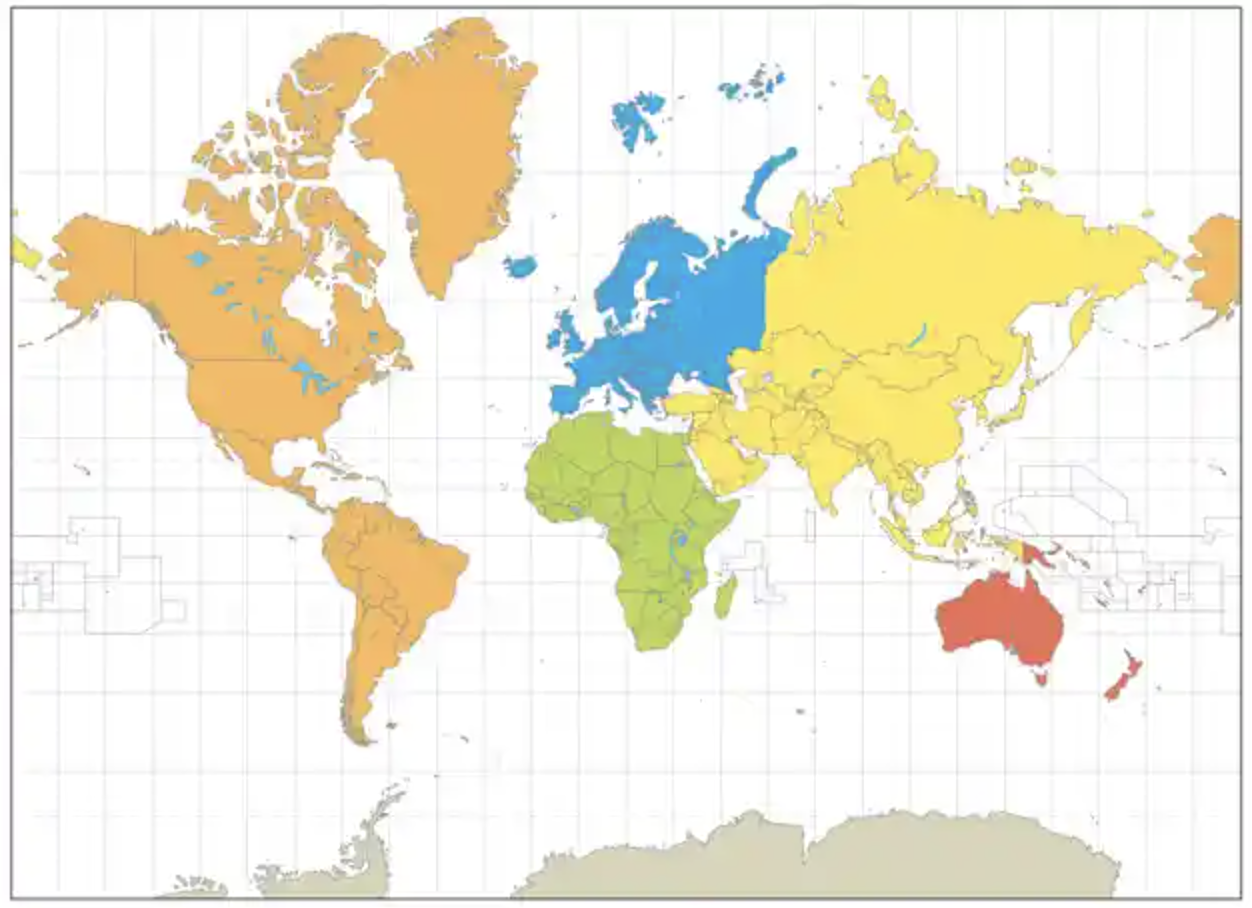
\includegraphics[width=0.7\linewidth]{Mercator.png}
            \caption{Mercator projection.}
            \label{fig:mappingsa}
        \end{subfigure}
        \begin{subfigure}[b]{0.3\linewidth}
            \centering
            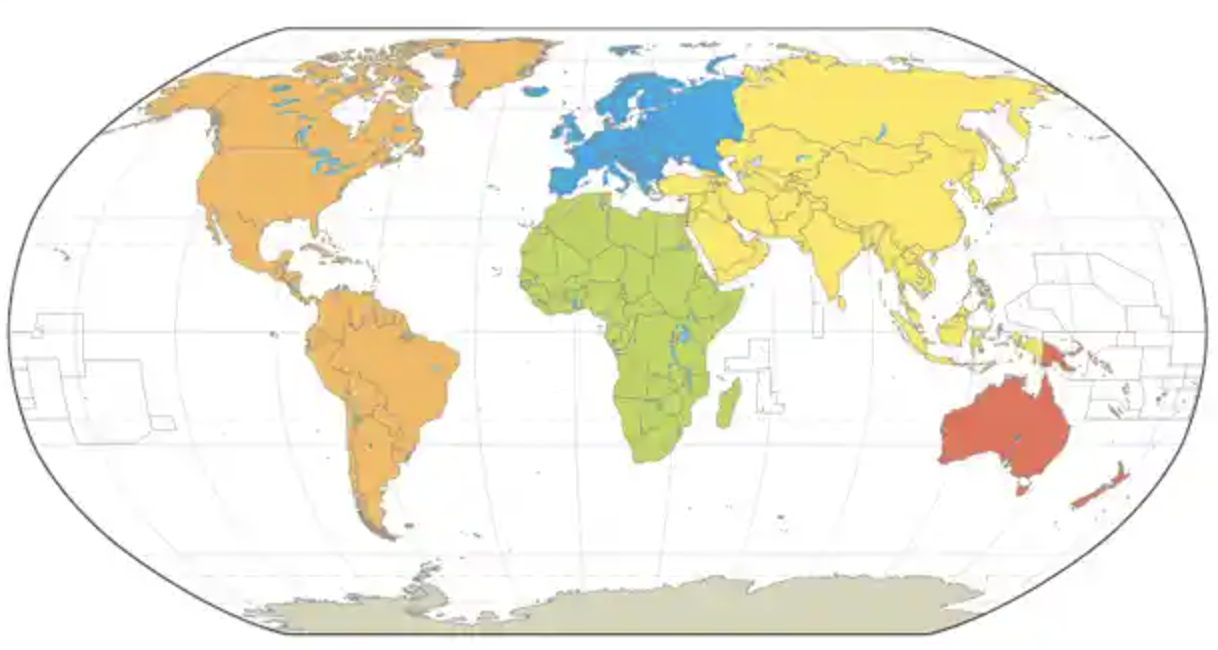
\includegraphics[width=0.9\linewidth]{Robinson.png}
            \caption{Robinson projection.}
            \label{fig:mappingsb}
        \end{subfigure}
        \begin{tikzpicture}[remember picture,overlay]
            \draw [ultra thick,-latex] (-5.8,1.8) -- ++(0.8,0);
        \end{tikzpicture}
        \caption{Visualizing functions of $\R^2\to\R^2$.}
        \label{fig:mappings}
    \end{figure}
    \vspace{-0.5em}
    \begin{itemize}
        \item What do these mappings do to the lines of latitude and longitude?
        \item This is a mapping of $\R^2\to\R^2$ that stretches and distorts! By drawing grid lines, we can see what it does to $\R^2$.
    \end{itemize}
    \item Now recall that $f$ holomorphic implies $Df$ looks like
    \begin{equation*}
        \begin{pmatrix}
            a & -b\\
            b & a\\
        \end{pmatrix}
    \end{equation*}
    \begin{itemize}
        \item What's nice about these matrices is they can always be factored into rotation and scaling matrices.
        \begin{equation*}
            \begin{pmatrix}
                a & -b\\
                b & a\\
            \end{pmatrix}
            =
            \begin{pmatrix}
                \cos\theta & -\sin\theta\\
                \sin\theta & \cos\theta\\
            \end{pmatrix}
            \begin{pmatrix}
                \lambda & 0\\
                0 & \lambda\\
            \end{pmatrix}
            \tag{$\lambda,\theta\in\R$}
        \end{equation*}
        \item This means that
        \begin{equation*}
            f'(z_0) = w = r\e[i\theta] \in \C
        \end{equation*}
        since multiplication by complex numbers also just rotates and scales!
        \item This means that if $z'=r'\e[i\theta']$, then $w\cdot z'=r\cdot r'\e[i(\theta+\theta')]$.
        \item This also means that we may have rotation and scaling but no shearing. Formally, we have the following lemma.
    \end{itemize}
    \item \textbf{Argument} (of $z\in\C$): The angle $\theta$ such that $z=r\e[i\theta]$ for some $r\in\R$. \emph{Denoted by} $\bm{\arg(z)}$.
    \item Lemma: Suppose two curves $\gamma,\delta$ intersect at a point $z\in\C$. Let $f:\C\to\C$ be holomorphic. Then
    \begin{equation*}
        \angle_z(\gamma,\delta) = \angle_{f(z)}(f(\gamma),f(\delta))
    \end{equation*}
    i.e., $f$ preserves angles.
    \begin{figure}[h!]
        \centering
        \begin{tikzpicture}[
            every node/.style=black
        ]
            \footnotesize
            \begin{scope}[xshift=-4cm]
                \draw [blx,thick,-latex] plot[smooth] coordinates
                    {(-0.5,-0.8) (-0.3,-0.4) (0,0) (0.5,0.2) (2,0) (2.5,0.5)}
                    node[right]{$\gamma$}
                ;
                \draw [rex,thick,-latex] plot[smooth] coordinates
                    {(-0.6,0.2) (-0.35,0.4) (0,0) (0.5,-0.6) (1,-1)}
                    node[right]{$\delta$}
                ;
                \draw [bly,semithick,->] (0,0) coordinate (z) -- (40:1) node[above right=-2pt]{$\gamma'(0)$};
                \draw [rey,semithick,->] (0,0) -- (-55:1) node[below left=-2pt]{$\delta'(0)$};
    
                \fill circle (1.5pt) node[left=1pt]{$z$};
            \end{scope}
            \draw [-stealth] (-1,1) to[bend left=20] node[above]{$f$} ++(2,0);
            \begin{scope}[xshift=2.5cm]
                \draw [blx,thick,-latex] plot[smooth] coordinates
                    {(-0.7,-0.8) (-0.4,-0.6) (0,0) (0.33,0.5) (1,0.7) (1.7,1.5)}
                    node[right]{$f(\gamma)$}
                ;
                \draw [rex,thick,-latex] plot[smooth] coordinates
                    {(-1,0) (-0.55,0.3) (0,0) (0.8,-0.3) (2,0.5) (2.5,0.3)}
                    node[right]{$f(\delta)$}
                ;
                \draw [bly,semithick,->] (0,0) -- (63:1) node[above]{$(f\circ\gamma)'(0)$};
                \draw [rey,semithick,->] (0,0) -- (-32:1) node[below right=-2pt]{$(f\circ\delta)'(0)$};
    
                \fill circle (1.5pt) node[left=1pt,yshift=-2pt]{$f(z)$};
            \end{scope}
        \end{tikzpicture}
        \caption{Holomorphic maps preserve angles.}
        \label{fig:holomorphicAngles}
    \end{figure}
    \begin{proof}
        To consider the angle between two curves analytically, let's look at the tangent vectors to the two curves, for example at $z$. Now while we often think of $\gamma'(0)$ as a \emph{matrix}, remember that we've proven that all of these matrices are equivalent to complex numbers. In particular, since $\gamma:\R\to\R^2\cong\C$, the total derivative will just be a vector. This vector may easily be represented as a complex number $r\e[i\theta]$ in polar coordinates. Similarly, $\delta'(0)$ can be thought of as a complex number $r'\e[i\theta']$. Thus, dividing these quantities gives us the angle $\theta-\theta'$ between the two vectors, which we can isolate using the argument function.\par
        Doing the same to the curves at $f(z)$ yields
        \begin{align*}
            \angle_{f(z)}(f(\gamma),f(\delta)) &= \arg\left[ \frac{(f\circ\gamma)'(0)}{(f\circ\delta)'(0)} \right]\\
            &= \arg\left[ \frac{f'(\gamma(0))\cdot\gamma'(0)}{f'(\gamma(0))\cdot\delta'(0)} \right]\\
            &= \arg\left[ \frac{f'(z)\cdot\gamma'(0)}{f'(z)\cdot\delta'(0)} \right]\\
            &= \arg\left[ \frac{\gamma'(0)}{\delta'(0)} \right]\\
            &= \angle_z(\gamma,\delta)
        \end{align*}
        as desired.
    \end{proof}
    \begin{itemize}
        \item Calderon gave us 5 minutes to try to compute this ourselves with the hint: Use the chain rule! $\angle_z(\gamma,\delta)=\arg(\gamma'(0)\cdot[\delta'(0)]^{-1})$.
    \end{itemize}
    \item \textbf{Conformal} (map): A function $f:U\to V$, where $U,V\subset\C$, that satisfies the following two constraints. \emph{Constraints}
    \begin{enumerate}
        \item $f$ is a diffeomorphism.
        \item $f$ preserves angles.
    \end{enumerate}
    \item \textbf{Diffeomorphism}: A homeomorphism for which $f,f^{-1}$ are differentiable.
    \item \textbf{Biholomorphic} (map): A function $f:U\to V$ that is bijective, holomorphic, and for which $f^{-1}$ is holomorphic.
    \item Theorem/observation: Biholomorphic iff conformal.
    \begin{proof}
        Follows straight from the definitions and the lemma we just proved.
    \end{proof}
    \item Calderon shows us an \href{https://wqferr.github.io/SimplyComplex/}{applet}.
    \begin{itemize}
        \item We can use the applet to help with the PSet, but we still do have to submit actual proofs.
        \item Allows you to visually see the lemma for instance.
        \item Example: Under $z\mapsto z^2$, the sector of radius 2 and argument $\pi/4$ goes to the sector of radius $2^2=4$ and argument $\pi/2$.
    \end{itemize}
\end{itemize}



\section{Chapter I: Analysis in the Complex Plane}
\emph{From \textcite{bib:FischerLieb}.}
\begin{itemize}
    \item \marginnote{3/19:}The preface only contains comments and instructions for an instructor planning to use this textbook for a course.
    \item The chapter begins with two paragraphs (as do all the others).
    \begin{itemize}
        \item The first discusses topic covered in the chapter.
        \item The second gives some historical background on these topics.
    \end{itemize}
\end{itemize}


\subsection*{Section I.0: Notations and Basic Concepts}
\begin{itemize}
    \item Goal: Reiew the fundamental topological and analytical concepts of real analysis.
    \item Defines the \textbf{complex numbers}, \textbf{complex plane}, and \textbf{complex conjugate}.
    \item \textbf{Absolute value} (of $z$): The Euclidean distance of $z$ from zero. \emph{Also known as} \textbf{modulus}. \emph{Denoted by} $\bm{|z|}$. \emph{Given by}
    \begin{equation*}
        |z| := \sqrt{x^2+y^2}
    \end{equation*}
    \item \textbf{Imaginary unit}. \emph{Denoted by} $\bm{i}$.
    \item Relating the modulus and complex conjugate.
    \begin{equation*}
        |z| = \sqrt{z\bar{z}}
    \end{equation*}
    \item \textbf{Open disk} (of radius $\varepsilon$ and center $z_0$): The set defined as follows. \emph{Also known as} \textbf{$\bm{\varepsilon}$-neighborhood} (of $z_0$). \emph{Denoted by} $\bm{D_\varepsilon(z_0)}$, $\bm{U_\varepsilon(z_0)}$. \emph{Given by}
    \begin{equation*}
        D_\varepsilon(z_0) = U_\varepsilon(z_0) := \{z\in\C:|z-z_0|<\varepsilon\}
    \end{equation*}
    \item \textbf{Unit disk}: The set defined as follows. \emph{Denoted by} $\pmb{\D}$. \emph{Given by}
    \begin{equation*}
        \D := D_1(0)
    \end{equation*}
    \item \textbf{Unit circle}: The set defined as follows. \emph{Denoted by} $\pmb{\Ss}$. \emph{Given by}
    \begin{equation*}
        \Ss := \{z\in\C:|z|=\varepsilon\}
    \end{equation*}
    \item \textbf{Upper half plane}: The set defined as follows. \emph{Denoted by} $\pmb{\Hh}$. \emph{Given by}
    \begin{equation*}
        \Hh := \{z\in\C:\im z>0\}
    \end{equation*}
    \item $\bm{\pmb{\C}^*}$: The set defined as follows. \emph{Given by}
    \begin{equation*}
        \C^* := \C\setminus\{0\}
    \end{equation*}
    \item \marginnote{3/21:}\textbf{Neighborhood} (of $z_0$): A set $U$ which contains an $\varepsilon$-neighborhood.
    \item \textbf{Open} (set): A set that is a neighborhood of each of its points.
    \item \textbf{Closed} (set): A complement of an open set.
    \item \textbf{Interior} (of $M$): The largest open set contained in $M$. \emph{Denoted by} $\bm{\mathring{M}}$.
    \item \textbf{Closure} (of $M$): The smallest closed set containing $M$. \emph{Denoted by} $\bm{\overline{M}}$.
    \item \textbf{Topological boundary} (of $M$): The set defined as follows. \emph{Also known as} \textbf{boundary}. \emph{Denoted by} $\bm{\partial M}$. \emph{Given by}
    \begin{equation*}
        \partial M := \overline{M}\setminus\mathring{M}
    \end{equation*}
    \item \textbf{Relatively open} (set in $M$): The intersection of an open set $U$ with an arbitrary set $M$. \emph{Also known as} \textbf{open} (set in $M$).
    \item \textbf{Relatively closed} (set in $M$): The intersection of a closed set $U$ with an arbitrary set $M$. \emph{Also known as} \textbf{open} (set in $M$).
    \item \marginnote{4/4:}\textcite{bib:FischerLieb} define \textbf{convergent series} and their \textbf{limits} in the usual way.
    \begin{itemize}
        \item Sum, product, and reciprocal rules stated.
    \end{itemize}
    \item \textbf{Accumulation point} (of $M\subset\C$): A point $z_0\in\C$ for which there is a sequence $\{z_n\}\subset M\setminus\{z_0\}$ with $\lim z_n=z_0$.
    \item \textbf{Bounded} (set): A set $K$ for which $|z|\leq R$ for some $R$ and all $z\in K$.
    \item \textbf{Compact} (set): A closed, bounded set.
    \begin{itemize}
        \item Each sequence in a compact set contains convergent subsequences with limit in the set.
    \end{itemize}
    \item \textbf{Relatively compact} (set in $V$): A set $U$ for which $\overline{U}$ is a compact subset of $V$. \emph{Denoted by} $\bm{U\subset\subset V}$.
    \item Definition of a \textbf{complex-valued function}.
    \item \textbf{Continuous} (function at $z_0$): A function $f:U\to\C$ such that for each neighborhood $M$ of $w_0=f(z_0)$, there is a neighborhood $N$ of $z_0$ with $f(U\cap N)\subset M$; equivalently, the following holds true for all convergent sequences $\{z_n\}\subset U$.
    \begin{equation*}
        f\left( \lim_{n\to\infty}z_n \right) = \lim_{n\to\infty}f(z_n)
    \end{equation*}
    \item \textbf{Real part} (of $f:U\to\C$): The real-valued function $g$ such that $f=g+ih$.
    \item \textbf{Imaginary part} (of $f:U\to\C$): The complex-valued function $h$ such that $f=g+ih$.
    \item Continuity results.
    \begin{itemize}
        \item $f$ is continuous iff its real and imaginary parts are.
        \item The \textbf{composition} of continuous functions is continuous.
        \item Example of a continuous function: Any polynomial in $z,\bar{z}$, i.e., any function of the form
        \begin{equation*}
            f(z) = \sum_{j,k=0}^Na_{jk}z^j\bar{z}^k
        \end{equation*}
    \end{itemize}
    \item \textbf{Path}: A continuous map from a closed finite interval into the complex plane. \emph{Denoted by} $\bm{\gamma:[a,b]\to\pmb{\C}}$.
    \begin{itemize}
        \item We say that $\gamma$ \textbf{connects} its \textbf{initial point} and \textbf{end point}.
    \end{itemize}
    \item \textbf{Trace} (of a path): The image set $\gamma([a,b])$. \emph{Denoted by} $\bm{\textbf{tr}\,u}$.
    \item \textbf{Initial point} (of a path): The point $\gamma(a)$.
    \item \textbf{End point} (of a path): The point $\gamma(b)$.
    \item \textbf{Connected} (set): A set $U$ for which any two points of $U$ can be connected by a path whose trace lies in $U$. \emph{Also known as} \textbf{pathwise connected}.
    \item \textbf{Domain}: A connected open set.
    \begin{itemize}
        \item "An open set $U$ is a domain if and only if no decomposition of $U$ into disjoint nonempty subsets exists" \parencite[3]{bib:FischerLieb}.
    \end{itemize}
    \item Images of compact (resp. connected) sets under continuous functions are again compact (resp. connected).
    \item Images of open (resp. closed) sets under continuous functions are \emph{not necessarily} open (resp. closed).
    \item Preimages of open (resp. closed) sets under continuous functions are again open (resp. closed).
    \item Note that the above definitions make sense in higher-dimensional vector spaces upon replacing the absolute value with the \textbf{Euclidean norm}.
\end{itemize}


\subsection*{Section I.1: Holomorphic Functions}
\begin{itemize}
    \item \marginnote{4/5:}Definition of \textbf{holomorphic}.
    \item Examples and nonexamples of holomorphic functions: Constant, identity, and complex conjugate functions.
    \item Further comments on the complex conjugate function.
    \begin{itemize}
        \item It's everywhere continuous but nowhere complex differentiable.
        \item It's very hard to find real examples of such functions, but we found a complex example like that!
    \end{itemize}
    \item For the basic properties of complex differentiation (e.g., holomorphic implies continuous, sum and product rules), the proofs are symmetric to the real ones.
    \item $\mO(U)$ is a ring, but it is more technically a $\C$-algebra.
    \item \textbf{Chain rule}: If $f:U\to V$ and $g:V\to\C$ are mappings of open subsets of $\C$ that are holomorphic at $z_0\in U$ and $f(z_0)=w_0\in V$, respectively, then $g\circ f:U\to\C$ is holomorphic at $z_0$ and
    \begin{equation*}
        (g\circ f)'(z_0) = g'(w_0)f'(z_0)
    \end{equation*}
    \item Definition of \textbf{biholomorphic}.
    \item \textcite{bib:FischerLieb} prove some elementary properties of complex functions in places with nonzero derivatives (e.g., locally one-to-one).
    \begin{itemize}
        \item This leads into the \textbf{complex inverse function theorem}.
        \item Preview: This leads to the result that "bijective holomorphic maps are biholomorphic," i.e., if we have a bijective holomorophic map, we don't also need to prove that $f^{-1}$ is holomorphic \parencite[6]{bib:FischerLieb}.
    \end{itemize}
\end{itemize}


\subsection*{Section I.2: Real and Complex Differentiability}
\begin{itemize}
    \item Definition of \textbf{$\bm{\pmb{\R}^2}$-differentiable function}.
    \item Definition of \textbf{Wirtinger derivatives}.
    \begin{itemize}
        \item \textcite{bib:FischerLieb} arrive here from a slightly different angle than in class.
    \end{itemize}
    \item \textcite{bib:FischerLieb} prove the $\pdv*{f}{\bar{z}}=0$ condition.
    \item \textbf{Cauchy-Riemann operator}: The differential operator defined as follows. \emph{Denoted by} $\bm{\partial/\partial\bar{z}}$. \emph{Given by}
    \begin{equation*}
        \pdv{\bar{z}} := \frac{1}{2}\left( \pdv{x}+i\pdv{y} \right)
    \end{equation*}
    \item "In requiring that a function be complex differentiable we thus simultaneously require
    that a certain partial differential equation be satisfied. In other words, \emph{holomorphic
    functions are the differentiable solutions of the Cauchy-Riemann equation}" given as follows \parencite[9]{bib:FischerLieb}.
    \begin{equation*}
        {\pdv{f}{\bar{z}}}(z) = 0
    \end{equation*}
    \item \textbf{Laplace operator}: The real differential operator defined as follows. \emph{Also known as} \textbf{Laplacian}. \emph{Denoted by} $\bm{\Delta}$. \emph{Given by}
    \begin{equation*}
        \Delta := \pdv[2]{x}+\pdv[2]{y}
    \end{equation*}
    \begin{itemize}
        \item As a real differential operator,
        \begin{equation*}
            \Delta\bar{f} = \overline{\Delta f}
        \end{equation*}
        \item More on this operator in Section VII.6.
    \end{itemize}
    \item Definition of a \textbf{harmonic function}, the \textbf{Cauchy-Riemann equations} (in real form).
    \item On the CR equations: "The gradients and, consequently, the equipotential lines of g and h are thus perpendicular to one another at all points where the gradients do not vanish" \parencite[10]{bib:FischerLieb}.
    \item We now investigate a special case of the chain rule for the Wirtinger derivatives.
    \item Lemma 2.4: Let $f:U\to\C$ be a real differentiable function defined on an open set $U\subset\C$ and let $w:[a,b]\to U$ be a differentiable map (i.e., a differentiable path in $U$). Then for all $t\in[a,b]$,
    \begin{equation*}
        \pdv{t}(f\circ w)(t) =
        \begin{pmatrix}
            f_z(w(t)) & f_{\bar{z}}(w(t))\\
        \end{pmatrix}
        \begin{pmatrix}
            \dot{w}(t)\\
            \dot{\bar{w}}(t)\\
        \end{pmatrix}
        = f_z(w(t))\dot{w}(t)+f_{\bar{z}}(w(t))\dot{\bar{w}}(t)
    \end{equation*}
    Here we denote $\pdv*{w}{t}$ by $\dot{w}$ and use matrix multiplication.
    \begin{proof}
        Left to the reader.
    \end{proof}
    \item \textbf{Complex linear map}: A map $l:\C\to\C$ characterized by the following. \emph{Constraints}
    \begin{enumerate}
        \item $l(z+w)=l(z)+l(w)$;
        \item $l(rz)=rl(z)$;
    \end{enumerate}
    for $z,w,r\in\C$.
    \begin{itemize}
        \item Every complex linear map is of the form
        \begin{equation*}
            w = l(z) = az
        \end{equation*}
        for a unique $a\in\C$.
    \end{itemize}
    \item \textbf{Real linear map}: A map $l:\C\to\C$ characterized by the following. \emph{Constraints}
    \begin{enumerate}
        \item $l(z+w)=l(z)+l(w)$;
        \item $l(rz)=rl(z)$;
    \end{enumerate}
    for $z,w\in\C$ and $r\in\R$.
    \begin{itemize}
        \item Every real linear map is of the form
        \begin{equation*}
            w = l(z)
            = az+b\bar{z}
            =
            \begin{pmatrix}
                a & b\\
            \end{pmatrix}
            \begin{pmatrix}
                z\\
                \bar{z}\\
            \end{pmatrix}
        \end{equation*}
        for a unique pair $
            \begin{pmatrix}
                a & b\\
            \end{pmatrix}
            \in\C^2
        $.
        \item Implication: $l$ is complex linear iff $b=0$.
    \end{itemize}
    \item \textbf{Tangent map} (of $f$ at $z_0$): The real linear map from $\C\to\C$ determined by the vector $
        \begin{pmatrix}
            f_z(z_0) & f_{\bar{z}}(z_0)\\
        \end{pmatrix}
    $.
    \item Proposition: $f$ is holomorphic at $z_0$ iff its tangent map at $z_0$ is complex linear.
    \item \textcite{bib:FischerLieb} discuss angle preservation, per Figure \ref{fig:holomorphicAngles}.
\end{itemize}




\end{document}